\chapter{Introduction to Vectors}
% Alternate title: Vectors and their Mathematical Operations

{
\begin{center}
\fcolorbox{black}{shadecolor}{%

    \parbox{\textwidth}
    {%
        \small
        {
            This chapter is a basic introduction to vectors their mathematical operations. If you have already studied them, feel free to proceed to the next chapter!
        }
    }%
}
\end{center}
}

Whenever we want to define a quantity, we use numbers. For instance, if someone asks you how many candies you have, you can answer them in forms of numbers, say 1, 5, or 100. Numbers let you have a concrete idea about the amount of things. Thus, if you know that you have 5 candies and your sibling has 2, you can be sure that you have more candies than your sibling (yay!). The number which describe the 'quantity' of something is called its \textbf{magnitude}.

In science, we call all such things \textbf{scalar}. Because of this, we can say that a scalar is a quantity that can be described alone by its magnitude.

Let's take another example now. Suppose someone is asking you how far your school is from your home. You will make a nice guess and again answer in some sort of number, say 1 mile or 2 kilometers. That's all good -- no one will want you to \textit{measure} the whole distance on your own anyway. But there's still a problem. Even if we know that the school is 1 mile away from your home, this does not \textit{completely} describe the location of the school, because the school could either be in the north, south, east, or west of your home -- or anywhere in between. Hence, magnitude alone is not enough to describe the position of your school.

\begin{figure}[ht!]
    \centering
    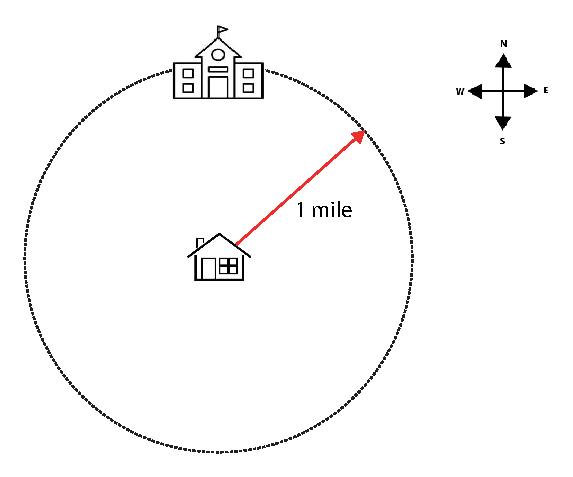
\includegraphics[scale = 0.7]{direction.eps}
    \caption{The problem faced with describing the position of the school from home. Every point on the circle is 1 mile away from the home, so saying 'My school is 1 mile away from home' is not enough; you need to tell the direction as well. In this figure, the direction is north.}
    \label{fig:direction}
\end{figure}

This problem demands that we add \textbf{direction} to our description as well. Hence, if you say that your school is 1 mile north from your home, this will completely describe the location of your school from your home. That is, we can say that position is completely described by both magnitude and direction. 

These quantities are called \textbf{vectors}. Thus, a vector is a physical quantity that is completely described by its magnitude and direction (and please keep this in mind; vectors will be your best bud to understand the next chapters!).

All the physical quantities are either scalars or vectors, about which you will study in your high school physics. But for now, this much description will be sufficient for the rest of the book.

\section{Description of Vector}
Just like we use numbers to describe scalars, we have different systems to describe vectors. 
\subsection{Polar Representation}
I'll be referring back to Fig. \ref{fig:direction}. Let's look at it from a different perspective. In the image, the magnitude of the position is given as the radius of the circle (in our case: 1 mile). So, all we need to do is describe the direction. For that, we will use angles. Suppose we take east as 0\si{\degree}. In that case, north will be described as 90\si{\degree} away from it. Thus, in polar representation, our position vector can be written as $1\phase{90\si{\degree}}$ mile. This is shown in Fig. \ref{fig:polar}.

\begin{figure}[!ht]
    \centering
    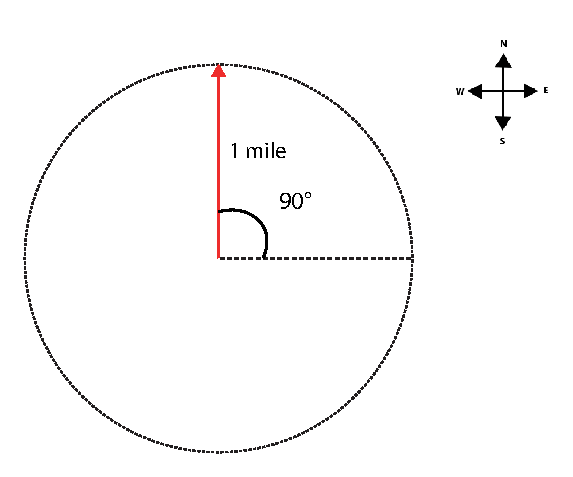
\includegraphics[scale = 0.8]{polar.eps}
    \caption{Redefining Fig. \ref{fig:direction} to show that the position vector can be represented with a radius and an angle, otherwise known as the polar representation of vectors. The images of house and school have been removed for convenience}
    \label{fig:polar}
\end{figure}

Generally speaking, the polar representation of a vector comprises a magnitude $r$ and an angle $\theta$; the vector itself is written as $r\phase{\theta}$.

\subsection{Rectangular Representation}
% write about (x, y) coordinates
Let's look back at Fig. \ref{fig:direction}. In fact, let's bring it on an x-y plane as shown in Fig. \ref{fig:rect-vec}. Here, we can see that the coordinates of the school are (0,10) if we consider one big box (marked by a slightly bolder grey line on the grid) as 0.1 mile. We can write this in vector notation as 10 $\hat{y}$ miles. Here, $\hat{y}$ simply means that this is the y-component of the vector. The meaning of the hat will be described shortly.

\begin{figure}[!ht]
    \centering
    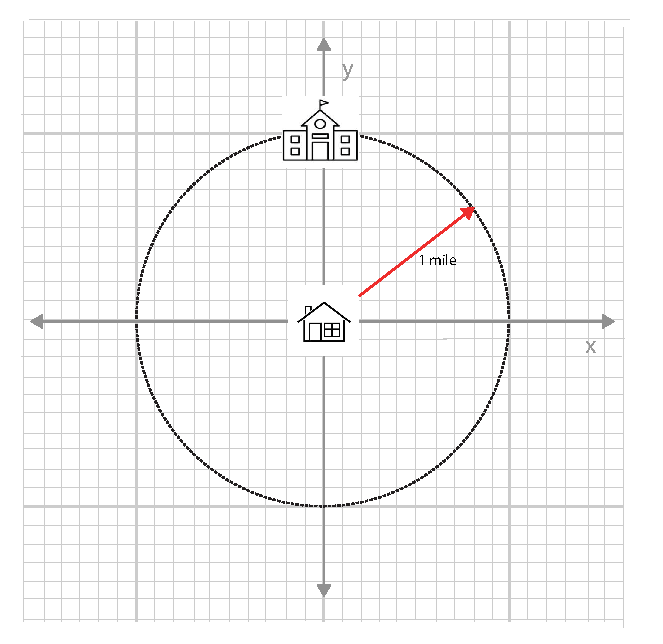
\includegraphics[scale = 0.7]{rect-vec.eps}
    \caption{Caption}
    \label{fig:rect-vec}
\end{figure}

Similarly the coordinates of the red vector are (8, 6) and we can write this as 8$\hat{x}$ + 6$\hat{y}$ miles. 

Hence, we are describing the vectors as a sum of an x-directed vector $\hat{x}$ and a y-directed vector $\hat{y}$. This can be written as $x \hat{x} + y\hat{y}$ where $x$ and $y$ are the x and y components of the vector respectively. 

%Here, the magnitude of the distance remains unchanged if we consider one big box (marked by a slightly bolder grey line on the grid) as one mile. As for the direction, we see that the school is on the y-axis. So, the position of the school can be written as 1 $\hat{y}$ mile. I will explain the meaning of $\hat{y}$ shortly; for now, just believe me that it means that the vector is magnitude 1 in y-axis.
There are some other ways of describing vectors as well, which we will explore in the last section. In the meantime, let's briefly see all the wonders we can do with vectors!

\section{Further Insights Into Vectors}
\subsection{Unit Vector}
We have just seen what magnitude is -- in simple words, it shows us how long a segment is. As you may have noticed, we used some letters with a "hat" to name the vectors of the previous examples (such as $\hat{x}$ and $\hat{y}$). And no -- we did not put them in that way for nothing! It is a special notation for \textbf{unit vectors}.

A unit vector, as its name states, has a \textbf{magnitude of 1}. That's the only requirement! This type of vector is usually denoted with a lowercase letter with a "hat", just like this:
%put an image with a unit vector and an a-hat

For example, v = (-3/5, 4/5) is a unit vector because: 

|v| = |(-3,5, 4/5)| = $\sqrt{(-3/5)^2 + (4/5)^2} = \sqrt{(9/25) + (16/25)} = \sqrt{25/25} = \sqrt{1} = 1$

{
\begin{center}
\fcolorbox{black}{shadecolor}{%

    \parbox{\textwidth}
    {%
        \small
        {
            \textbf{Fun Fact}:
            
            When you have a vector with the coordinates (0,0) it is called a \textit{zero vector}.
        }
    }%
}
\end{center}
}

\subsection{Conversion of Vector Representation}
As we mentioned before, vectors can be represented in diverse ways. In Fig. \ref{fig:polar} we explained polar representation; and on Fig. \ref{fig:rect-vec}, rectangular representation. 

On a not-so-random side note --could you imagine understanding a foreign language that you have never heard before \textit{without} a translator? Probably not. You would have to learn the brand new language to understand it by yourself. The very same things happens with different notations: sometimes, to understand them, we need to \textit{translate} them! Because of this, it is of utmost importance for you to know how to convert a vector from its polar form to its rectangular form and vice versa.

Here is an example: 
%put image of the example

Imagine you have a vector (2,2). This is written in its rectangular representation. However, if you observe really closely, you can realize that the diagram actually forms a right angle. This is \textbf{key} to know how to find the magnitude of the hypotenuse (in other words, the vector): the Pythagorean Theorem!

{
\begin{center}
\fcolorbox{black}{shadecolor}{%

    \parbox{\textwidth}
    {%
        \small
        {
            \textit{Side Note}: 
            The Pythagorean Theorem is a geometric theorem that uses the sum of the squares of both legs of the triangle to calculate the square of its hypotenuse. To put it in a simpler way, it follows the following formula: \[a^2 + b^2 = c^2\].
        }
    }%
}
\end{center}
}

If we apply the formula to our example, we would have the following mathematical calculations:

\begin{align*}
  2^2 + 2^2 &= c^2\\
  8 &= c^2\\
  \sqrt{8} &= c
\end{align*}

We now know that our hypotenuse's value is $\sqrt{8}$. As for the \textbf{angle}, we can find that using trigonometry. Since we know the three sides of the triangle, we can choose any trigonometric function we are most comfortable with. For this example, we will use \[\tan\theta = \frac{\text{opposite}}{\text{adjacent}}\]

So, for the tangent of this angle, it's \[\frac{2}{2} = 1\]

All we need to do now is take the inverse of that to have a final answer:

\[\theta = \tan^{-1}(1)\]
\[\theta = 45 ^{\circ}\]

\textbf{Congratulations!} You have now converted the vector's rectangular form into its polar form. The equality is as follows:

(2,2) = $\sqrt{8} \angle 45°$

And... \textit{what if we want to go the other way around? What if I want to convert a polar representation to a rectangular representation?}. That is a matter of simple trigonometry as well! 

%add image

To understand this, another brief example is this vector with magnitude r and an angle $\theta$. The \textbf{x coordinate} is \[r \cos\theta\] and the \textbf{y coordinate} is \[r \sin \theta\]. Thus, we can take some formulas to make the conversion process much faster:
\[r \angle \theta = (r \sin \theta, r \cos \theta)\]

Pretty simple, right? If there are any problems with the complex calculations (or short time), remember calculators are always there to help!

We are now masters of converting polar to rectangular forms but, how do we \textit{normally} operate with vectors? This topic will be discussed in the next section.

\section{Operations on Vectors}
With the extension of elementary algebra to vectors, we can now introduce \textbf{vector operations}.
\subsection{Addition}
Let's first consider vector $\overrightarrow{v}$ and  $\overrightarrow{w}$.
%draw both vectors with the tip-to-tail or parallelogram method

$\overrightarrow{v}$ + $\overrightarrow{w}$ is defined to be the resultant vector that goes from the tail of $v$ to the head of $w$. 
%drawing that pictures the sum
\subsection{Subtraction}
Another fun fact! Some mathematicians think that subtraction \textbf{does not exist}. Instead, it's just the inverse operation of addition. Thus, if we want to subtract $\overrightarrow{v}$ - $\overrightarrow{w}$, it could also be denoted as $\overrightarrow{v}$ + ($\overrightarrow{-w}$). With this concept, we can infer that the addition and subtraction of vectors are the same process -- just with a little \textit{twist}. The only difference is that we have to change the direction of the vector we are subtracting (in this case, $\overrightarrow{w}$). 
%put drawing 

\subsection{Scaling}
Before getting right into vector multiplication, we must first remember the unit vector. Why might this be useful? Well, vectors can be "scaled" off the unit vector. For example, vector a is shown to be 2,5 times a unit vector. 
%put image

\subsection{Multiplication}
Expanding more on scaling, this process is solely based on scalar multiplication. As you could see, a scalar multiplier k$>$0 can change the magnitude of the vector but not its direction. If k $<$ 0, then the scalar product will "reverse" the direction by 180 degrees.

For example, in rectangular form, if k is a scalar then
\[k(a,b) = (ka, kb)\]

\section{More Ways of Describing Vectors}
\subsection{Matrix Notation}
If you want to take your knowledge to the next level on vector notation, this is the right place to start! 

Matrices are defined as a rectangular array of numbers arranged in \textit{rows} and \textit{columns}. These numbers are called \textbf{elements}. Thus, the dimension of the matrix below is 2 x 3, since there are two rows and three columns:
%put any 2 x 3 matrix

{
\begin{center}
\fcolorbox{black}{shadecolor}{%

    \parbox{\textwidth}
    {%
        \small
        {
            \textit{Fun fact}: 
            Matrices are widely applied in engineering, economics, and statistics as well as in many other fields of mathematics! 
        }
    }%
}
\end{center}
}

A matrix with a single row is called a \textit{row vector} and a matrix with a single column is called a \textit{column vector}. The elements in a matrix are usually represented by lower case letters with a single subscript (e.g., \[a_j, b_j, x_j\]). Some examples of both types of vectors are shown below:

3 x 1 column vector: \[v = [y_1, y_2, y_3]\]
1 x 4 row vector: \[w = [h_1 h_2 h_3 h_4]\]
\subsubsection{Basic Concepts of Matrices}
In addition to those concepts, here are other basic terms that any good mathematician must know! 
A \textbf{square matrix} has the exact same number of rows and columns. 
%put example

A \textbf{diagonal matrix} is a square matrix where the \textit{diagonal elements} (elements where the two subscripts are equal) are nonzero and the \textit{off-diagonal elements} are zero.
%put example

The \textbf{identity matrix} is a type of diagonal matrix where every single diagonal elements are equal to 1. This particular matrix is usually represented as I. 
%put example

A \textbf{symmetric matrix} is a square matrix where the jk\textsuperscript{th} element is equal to the kj\textsuperscript{th} element.
%put example of 3x3 matrix --> M = [14,5,2//5,20,8//2,8,11]

Last but definitely not least, a \textbf{one vector} is a row or column vector in which every element is equal to 1.
%example --> 1 = [1 1 1]
\subsubsection{Matrix Operations}
\subsubsection{Addition}
The first thing you must check when adding a pair of matrices is their order. \textbf{Both must have an identical order!} For example, if you have two matrices (A and B) of order 2x2, then their sum would be as follows:
%put example

\subsubsection{Subtraction}
Similarly to vectors, we can apply the concept of "subtraction as the opposite of addition", meaning that A - B = A + (-B). Specifically, we would have to subtract each element of one matrix from the corresponding element of the second matrix. An example that depicts this is the following:
%put example

\subsubsection{Scalar Multiplication}
If you want to multiply a scalar by a matrix, you have to multiply the scalar number by every element on the matrix. 
%put example

\subsubsection{Matrix Multiplication}
Multiplying matrices has just one requirement: the number of columns of the first matrix must be equal to the number of rows in the second matrix. To understand this better, here we have an example:
%put example

\subsubsection{Dot Product}
Imagine that you have a solar panel (we love sustainable energy sources!). As the sun moves through the sky, the angle between sunlight and the solar panel changes.
%put two images: one with the sun at a 90 degree angle w the solar panel and another paralleled placed to it (explained below)

As we can see in the image, it would be ideal if the sun hit the solar panel at a 90° angle so it could capture the most energy possible. On the other hand, if the sunlight is placed paralleled to the panel, then it could not get any significant energy from this source. With this case, we can conclude that \textbf{the angle between a pair of objects is important.}
 When this is the case, we have the dot product to help us out.
 
 The \textbf{dot product} is an operation on vectors that enables us to easily find the angle between two vectors. To make this calculation, it is important to note that when we talk about the angle between two vectors, we're picturing the vectors with \textit{their tails at the same point.}
 %put image of "two vectors" and the "angle between them"
 
To depict this definition in more detail, here we have an example:

If we have vectors v = (1,2,3) and w = (4,5,6); then v*w = (1)(4) + (2)(5) + (3)(6) = 32

As we can see, the dot product is an operation between two vectors that produces a \textbf{scalar}. And to turn this into degrees, there's a key property of the dot product:

\textit{If $\theta$ is the angle between v and w, then $v*w = |\abs{a}||\abs{b}| \cos\theta$} (Remember that ∥a∥ represents the length of a!)
 
Using this information, we can now find the angle between v and w. By the Pythagorean Theorem,
\[∥v∥ = \sqrt{1^2 + 2^2 + 3^2} = \sqrt{14}\]
\[∥w∥ = \sqrt{4^2 + 5^2 + 6^2} = \sqrt{77}\]

So, 
\[32 = (\sqrt{14})(\sqrt{77})cos \theta\]

Therefore,
\[cos \theta = \frac{32}{(\sqrt{14})(\sqrt{77})} = \frac{32}{7\sqrt{22}}\]

So,
\[\theta = arccos(\frac{32}{7\sqrt{22}})\]

\subsection{Dirac Notation}
Being, also called bra-ket notation, dirac notation used the angle brackets ($\langle$ and $\rangle$) and a vertical bar (|) to construct "bras" and "kets".

A \textbf{ket} denotes a vector in an abstract vector space. If we are talking in physical terms, kets also represent a state of a quantum system. A ket looks like this: "{$\displaystyle |v\rangle$ }" A common example is:
\[|\psi \rangle = \]

A \textbf{bra}, in short, denotes a linear form 